% Capítulo de fundamentação: MIMO massivo e equalização.
% Comentários CONTEÚDO/TEXTO/ESTADO vêm do esqueleto (rascunho_backbone.tex).

\chapter{MIMO massivo e equalização}\label{chap:mimo-equalizacao}
% Base geral, válida para qualquer receptor MIMO: o modelo do sistema, o canal
% e os equalizadores lineares. Termina no LMMSE e na SER, que o capítulo
% seguinte usa.
% Ordem: cada seção usa só o que veio antes.

\section{Modelo de sistema}\label{sec:sysmodel}
% CONTEÚDO  Uplink multiusuário: y = Hs + n; dimensões M, K; símbolos de uma
%           constelação (16-QAM, QPSK); E_s; SNR = 10 log10(E_s / sigma^2).
% TEXTO     1-noise-and-constraints.tex, "Uplink/Downlink" (11 linhas).
% ESTADO    parcial. "SNR" não aparece hoje no capítulo.

\subsection{Uplink/Downlink}

\begin{figure}[h]
    \caption{Descrição da Figura deve ir no topo}
    \begin{center}
        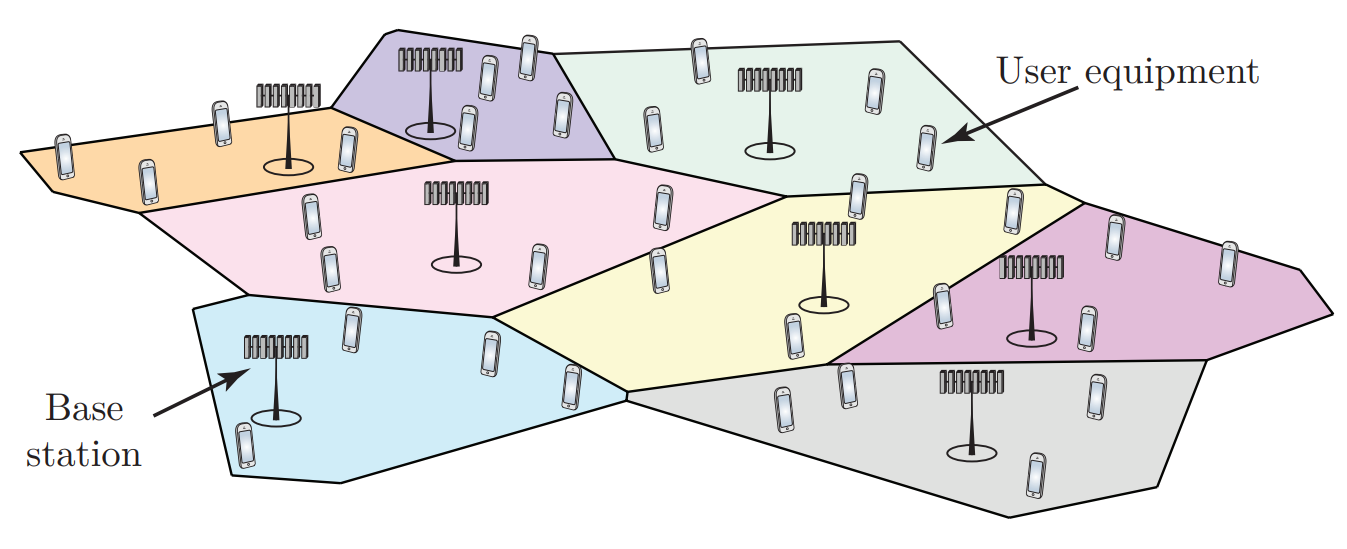
\includegraphics[width=0.7\textwidth]{Images/cell.png}
        % Aqui vai um includegraphics , um picture environment ou qualquer
        % outro comando necessário para incorporar o formato de imagem
        % utilizado.        
    \end{center}
    \label{fig:cell}
    \legend{Fonte: \cite{bjornson-mimo}}
\end{figure}


\subsection{Pilotos}
\subsection{Símbolos e constelação}

\subsection{Relação sinal-ruído}

\subsection{Detecção e taxa de erro de símbolo}
% Novo: decisão pelo ponto mais próximo da constelação; definição de SER.
